\documentclass{beamer}
\usepackage[english, russian]{babel}
\usepackage[T2A]{fontenc}
\usepackage[utf8]{inputenc}
\usepackage{indentfirst}
\usepackage{amsmath, amsfonts, amssymb, amsthm, mathtools}
\usepackage[export]{adjustbox}
\usepackage{graphicx} 
\graphicspath{ {./images/} }

\usepackage{subcaption}
\usepackage{verbatim}

\usepackage{minted}{\setlength{\parskip}{0pt}}

\usepackage{hyperref}

\hypersetup{
    colorlinks=true,
    linkcolor=blue,
    filecolor=magenta,      
    urlcolor=black,
    pdftitle={Overleaf Example},
    pdfpagemode=FullScreen,
    }


\title{Лабораторная работа № 16. \\ Базовая защита от атак типа "brute force"}
\author{Данила Стариков \\ НПИбд-02-22}
\institute{Российский университет дружбы народов имени Патриса Лумумбы}
\date{2024}

\begin{document}

\frame{\titlepage}

\begin{frame}
\frametitle{Цель работы}
\begin{itemize}
    \item Получить навыки работы с программным средством Fail2ban для обеспечения базовой защиты от атак типа "brute force".
\end{itemize}
\end{frame}

\begin{frame}[fragile]
\frametitle{Защита с помощью Fail2ban}
На сервере установили {\tt fail2ban}:
\begin{minted}{bash}
    dnf -y install fail2ban
\end{minted}
    \centering
    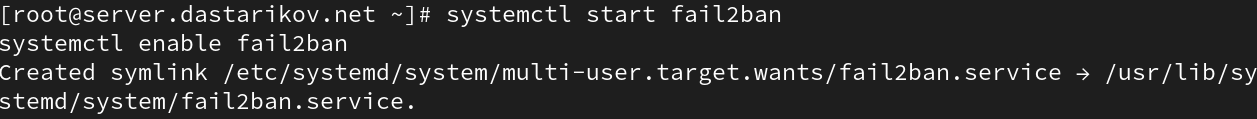
\includegraphics[width=\textwidth]{../images/image01.png}
    \captionof{figure}{Запуск сервиса \texttt{fail2ban}.}
\end{frame}

\begin{frame}
\frametitle{Защита с помощью Fail2ban}
    \centering
    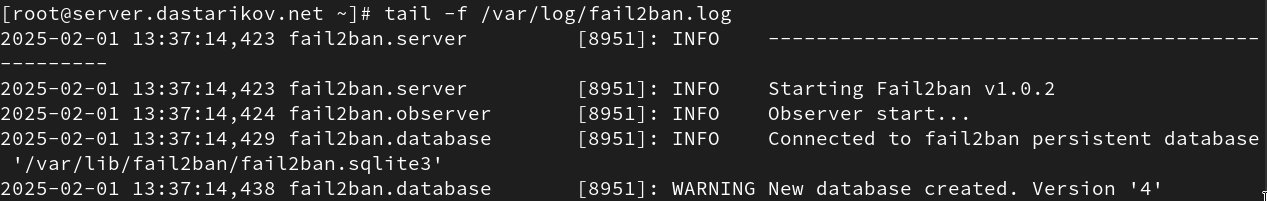
\includegraphics[width=\textwidth]{../images/image02.png}
    \captionof{figure}{Просмотр журнала событий \texttt{fail2ban}.}
\end{frame}

\begin{frame}[fragile]
\frametitle{Защита с помощью Fail2ban}
\begin{itemize}
\item Создали файл с новой конфигурацией {\tt fail2ban}:
\begin{minted}{bash}
    touch /etc/fail2ban/jail.d/customisation.local
\end{minted}
\item Задали время блокирования на 1 час (время задаётся в секундах):
\begin{minted}{bash}
      [DEFAULT]
      bantime = 3600
\end{minted}
  \item включили защиту SSH:
\begin{minted}{bash}
      [sshd]
      port = ssh,2022
      enabled = true
      [sshd-dos]
      filter = sshd
      enabled = true
      [selinux-ssh]
      enabled = true
\end{minted}
\end{itemize}
\end{frame}

\begin{frame}
\frametitle{Защита с помощью Fail2ban}
    \centering
    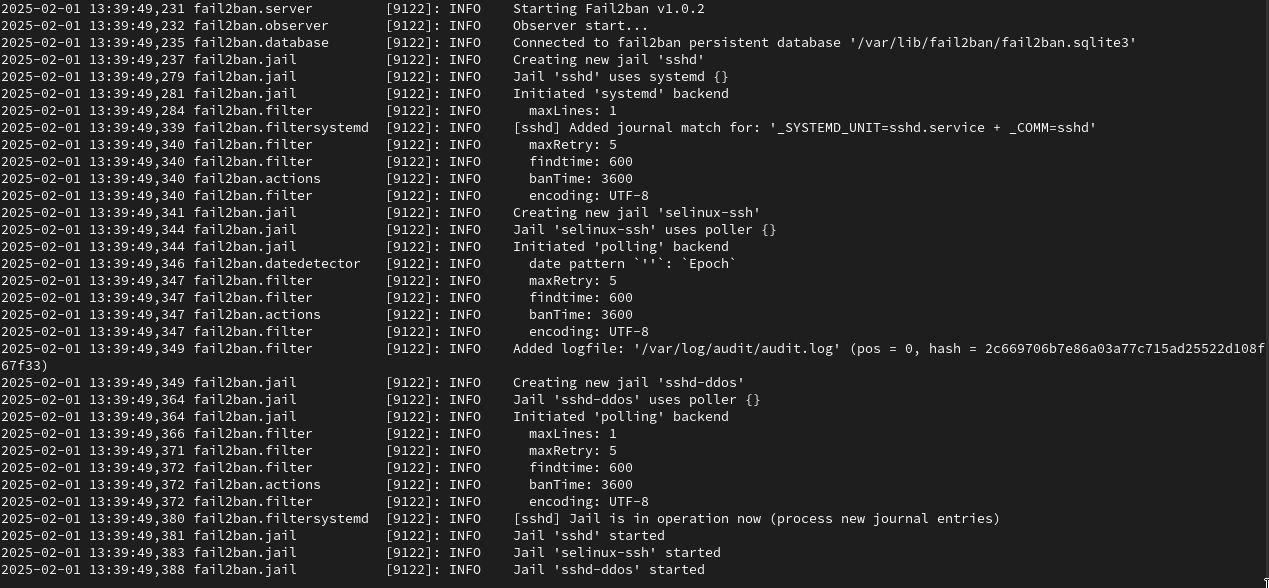
\includegraphics[width=\textwidth]{../images/image03.png}
    \captionof{figure}{Просмотр журнала событий после первоначальной настройки \texttt{fail2ban}.}
\end{frame}

\begin{frame}[fragile]
\frametitle{Защита с помощью Fail2ban}
В файле {\tt /etc/fail2ban/jail.d/customisation.local} включите защиту HTTP:
\begin{minted}[fontsize=\footnotesize]{bash}
    # HTTP servers
    [apache-auth]
    enabled = true
    [apache-badbots]
    enabled = true
    [apache-noscript]
    enabled = true
    [apache-overflows]
    enabled = true
    [apache-nohome]
    enabled = true
    [apache-botsearch]
    enabled = true
    [apache-fakegooglebot]
    enabled = true
    [apache-modsecurity]
    enabled = true
    [apache-shellshock]
    enabled = true
\end{minted}
\end{frame}

\begin{frame}
\frametitle{Защита с помощью Fail2ban}
    \centering
    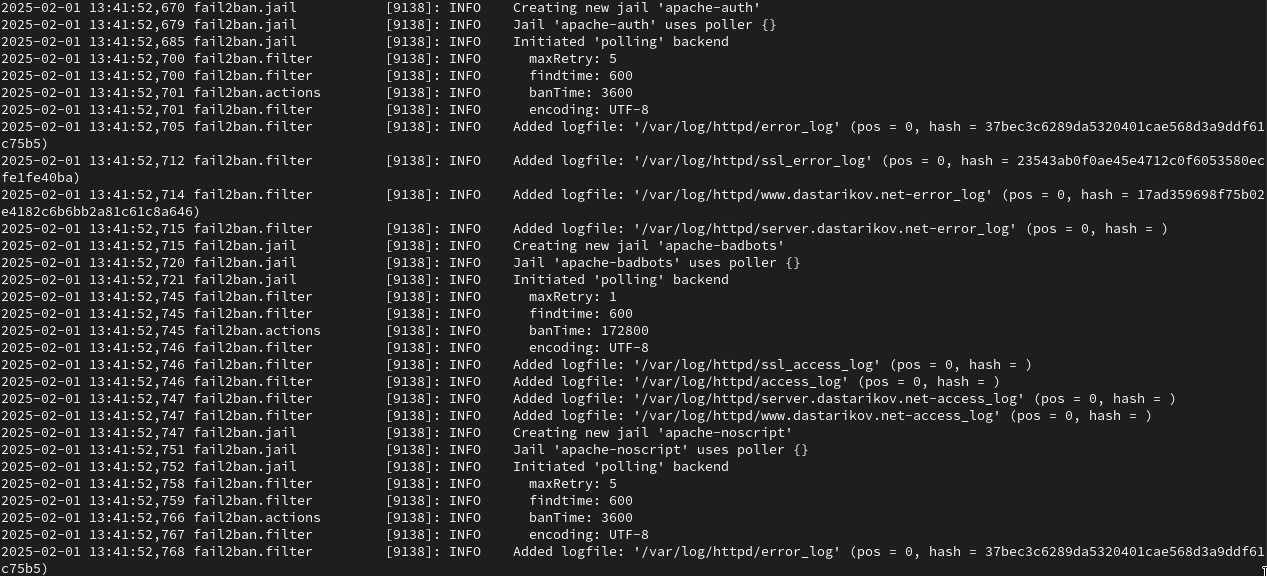
\includegraphics[width=\textwidth]{../images/image04.png}
    \captionof{figure}{Логи, связанные с защитой HTTP (Часть 1).}
\end{frame}

\begin{frame}
\frametitle{Защита с помощью Fail2ban}
    \centering
    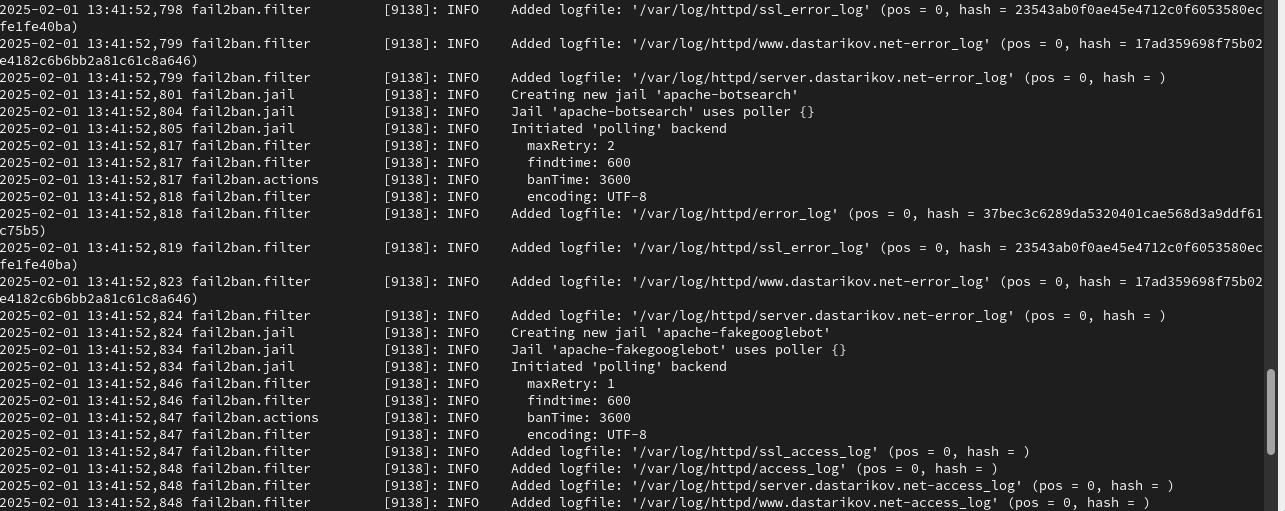
\includegraphics[width=\textwidth]{../images/image05.png}
    \captionof{figure}{Логи, связанные с защитой HTTP (Часть 2).}
\end{frame}

\begin{frame}
\frametitle{Защита с помощью Fail2ban}
    \centering
    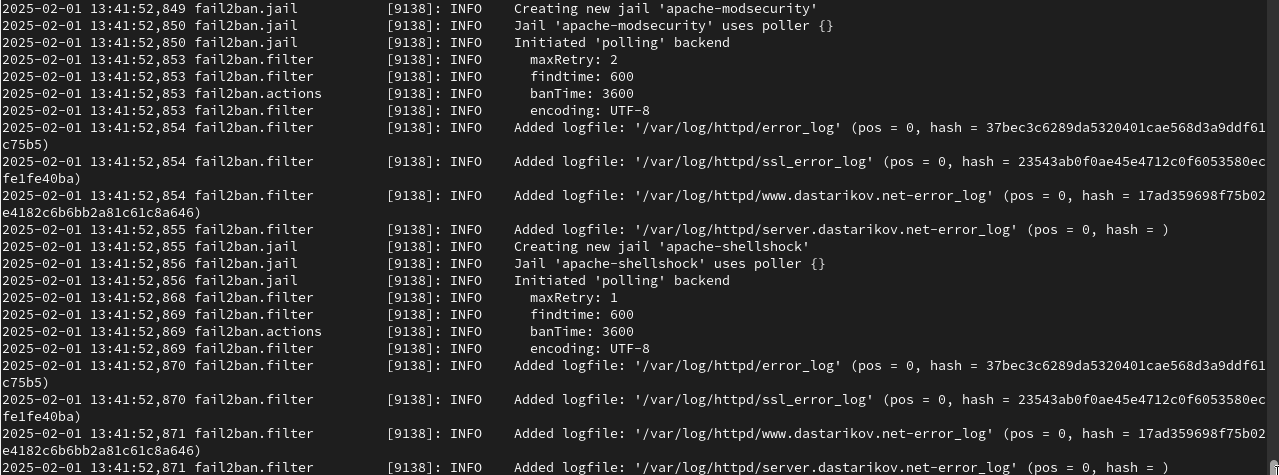
\includegraphics[width=\textwidth]{../images/image06.png}
    \captionof{figure}{Логи, связанные с защитой HTTP (Часть 3).}
\end{frame}

\begin{frame}[fragile]
\frametitle{Защита с помощью Fail2ban}
В файле {\tt /etc/fail2ban/jail.d/customisation.local} включите защиту почты:
\begin{minted}{bash}
    #
    # Mail servers
    #
    [postfix]
    enabled = true
    [postfix-rbl]
    enabled = true
    [dovecot]
    enabled = true
    [postfix-sasl]
    enabled = true
\end{minted}
\end{frame}

\begin{frame}
\frametitle{Защита с помощью Fail2ban}
  \centering
  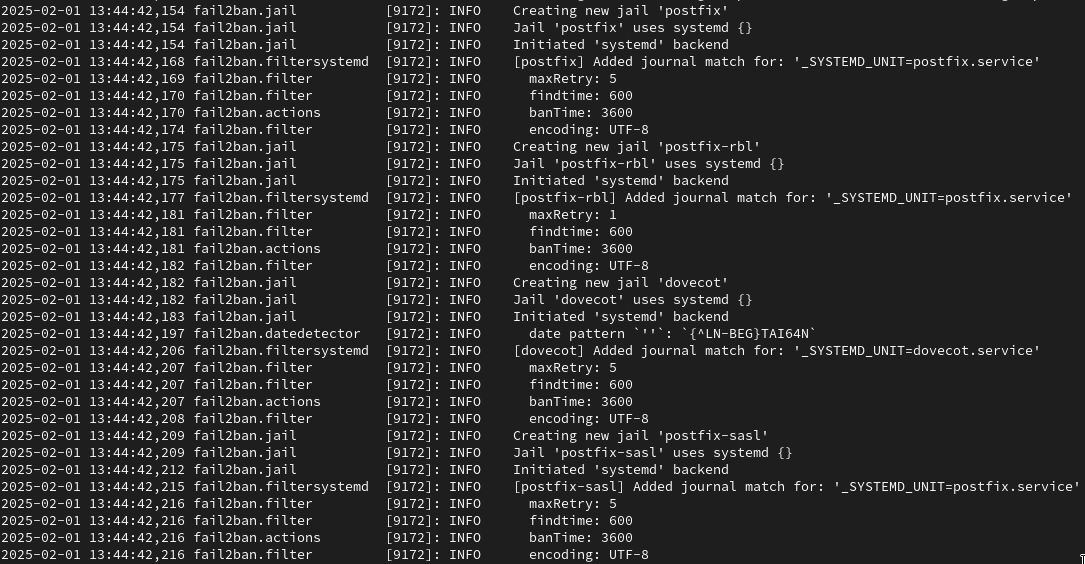
\includegraphics[width=\textwidth]{../images/image08.png}
  \captionof{figure}{Логи, связанные с защитой почты.}
\end{frame}


\begin{frame}
\frametitle{Проверка работы Fail2ban}
    \centering
    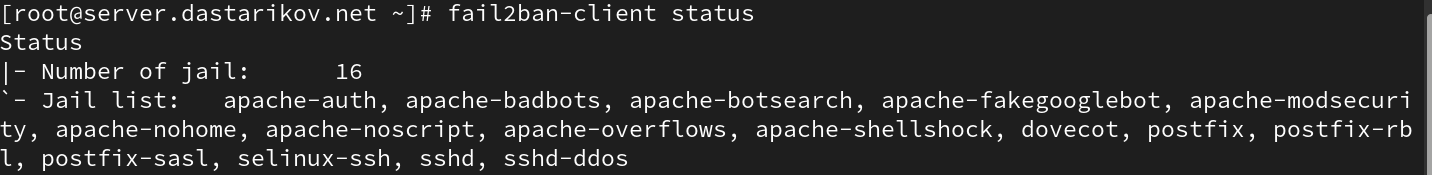
\includegraphics[width=\textwidth]{../images/image09.png}
    \captionof{figure}{Просмотр статуса \texttt{fail2ban}.}
\end{frame}

\begin{frame}
\frametitle{Проверка работы Fail2ban}
    \centering
    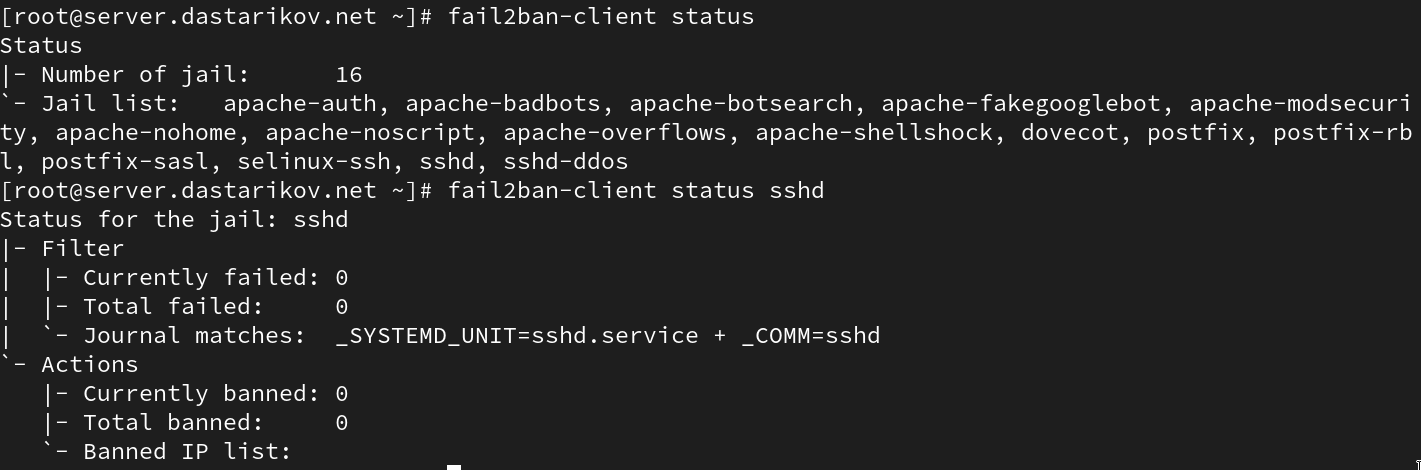
\includegraphics[width=\textwidth]{../images/image10.png}
    \captionof{figure}{Просмотр статуса защиты SSH.}
\end{frame}

\begin{frame}
\frametitle{Проверка работы Fail2ban}
    \centering
    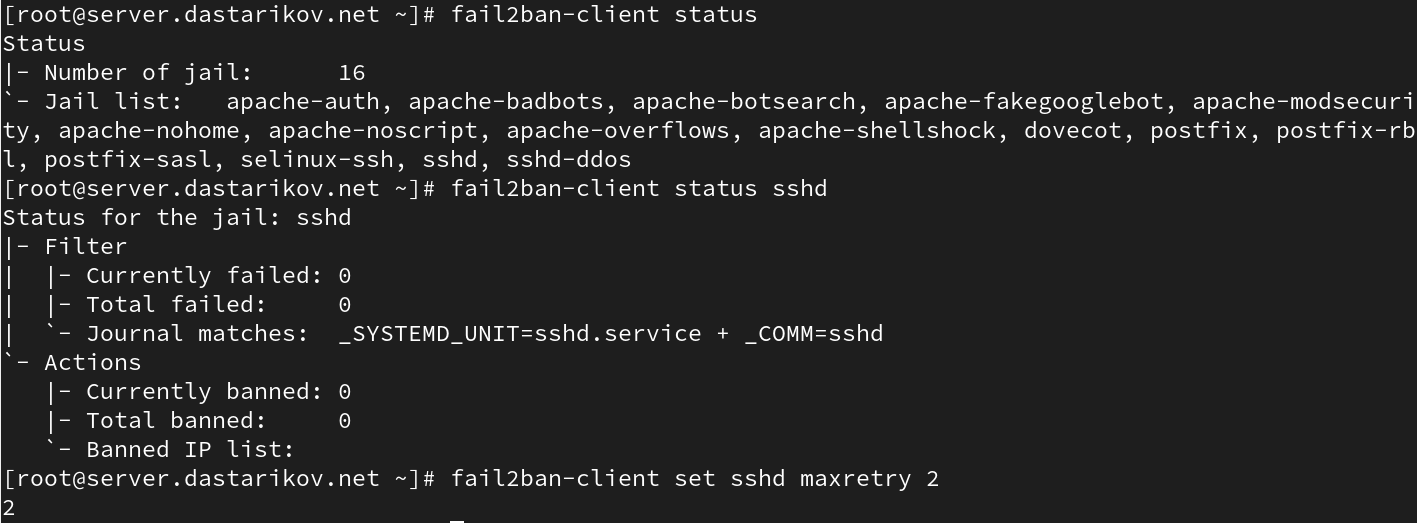
\includegraphics[width=\textwidth]{../images/image11.png}
    \captionof{figure}{Установка максимального количества ошибок для SSH.}
\end{frame}

\begin{frame}
\frametitle{Проверка работы Fail2ban}
    \centering
    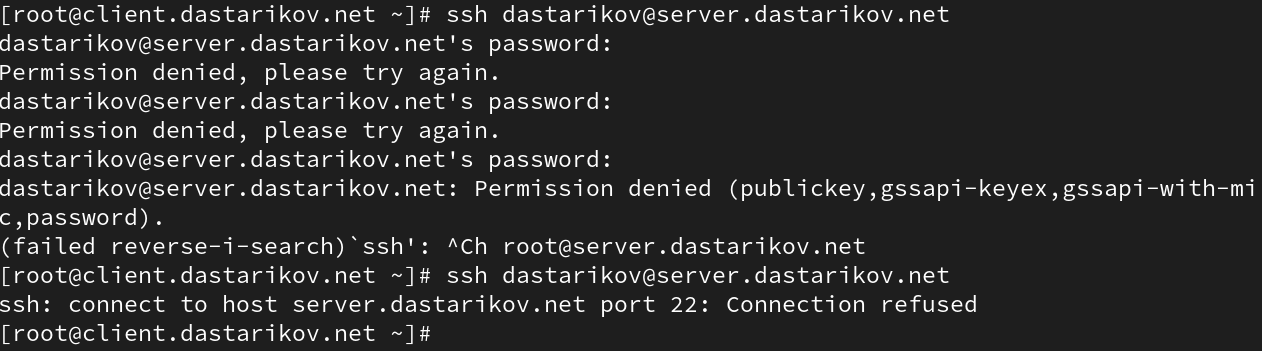
\includegraphics[width=\textwidth]{../images/image12.png}
    \captionof{figure}{Попытка зайти на сервер через SSH с неправильным паролем.}
\end{frame}

\begin{frame}
\frametitle{Проверка работы Fail2ban}
    \centering
    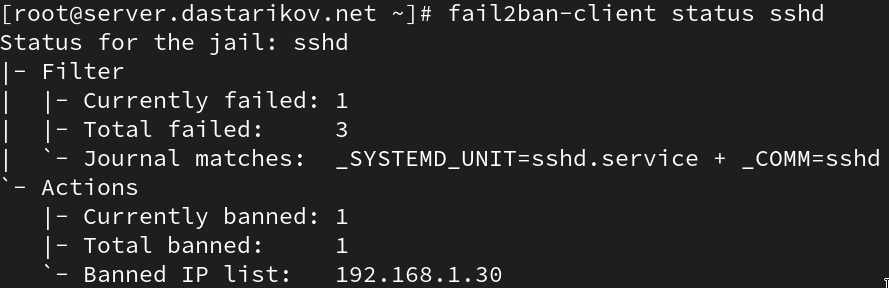
\includegraphics[width=\textwidth]{../images/image13.png}
    \captionof{figure}{Просмотр статуса защиты SSH.}
\end{frame}

\begin{frame}
\frametitle{Проверка работы Fail2ban}
    \centering
    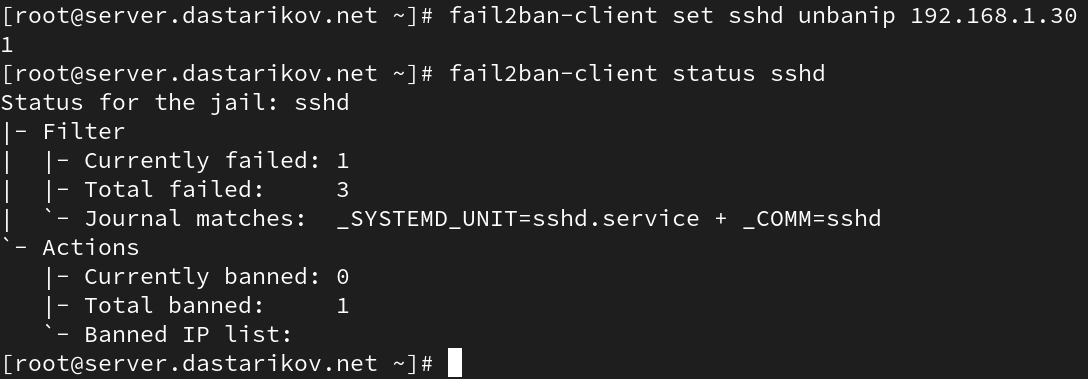
\includegraphics[width=\textwidth]{../images/image14.png}
    \captionof{figure}{Разблокировка ip-адреса клиента.}
\end{frame}

\begin{frame}
\frametitle{Проверка работы Fail2ban}
    \centering
    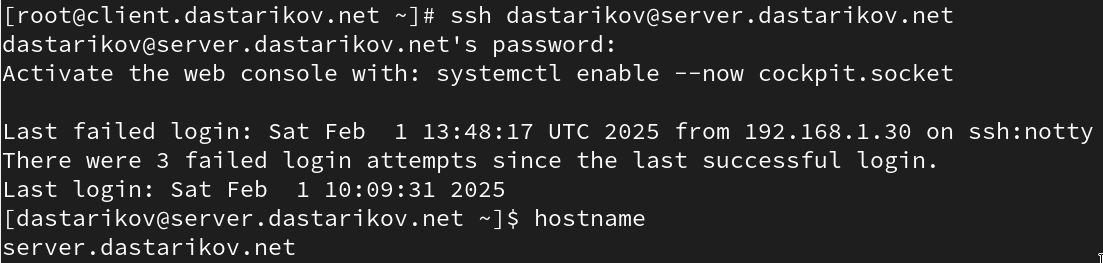
\includegraphics[width=\textwidth]{../images/image15.png}
    \captionof{figure}{Проверка снятия блокировки.}
\end{frame}

\begin{frame}[fragile]
\frametitle{Проверка работы Fail2ban}
На сервере внесли изменение в конфигурационный файл {\tt /etc/fail2ban/jail.d/customisation.local}, добавив в раздел по умолчанию игнорирование адреса клиента
\begin{minted}{bash}
    [DEFAULT]
    bantime = 3600
    ingoreip = 127.0.0.1/8 192.168.1.30
\end{minted}

    \centering
    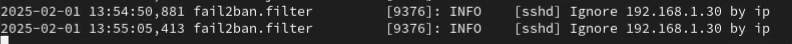
\includegraphics[width=\textwidth]{../images/image19.png}
    \captionof{figure}{Логи журнала об игнорировании адреса клиента.}
\end{frame}

\begin{frame}
\frametitle{Проверка работы Fail2ban}
    \centering
    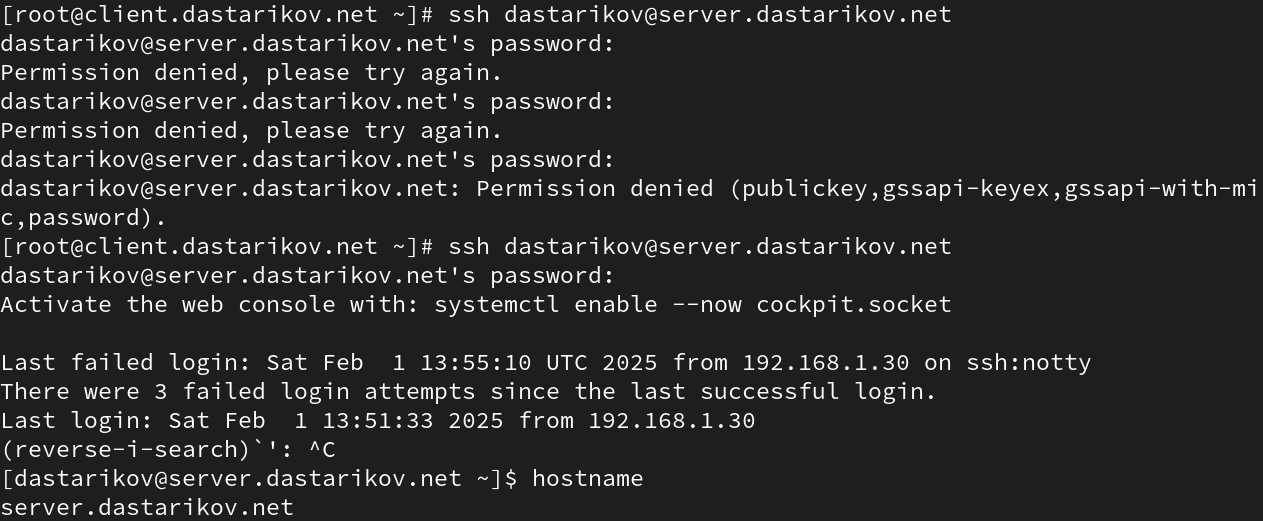
\includegraphics[width=\textwidth]{../images/image16.png}
    \captionof{figure}{Демонстрация игнорирования безуспешных попыток подключения по SSH.}
\end{frame}

\begin{frame}
\frametitle{Проверка работы Fail2ban}
    \centering
    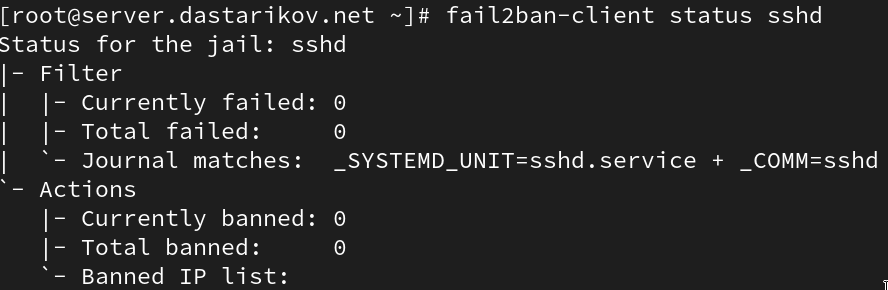
\includegraphics[width=\textwidth]{../images/image17.png}
    \captionof{figure}{Просмотр информации о защите SSH.}
\end{frame}




\begin{frame}
\frametitle{Внесение изменений в настройки внутреннего окружения виртуальных машин}
    \centering
    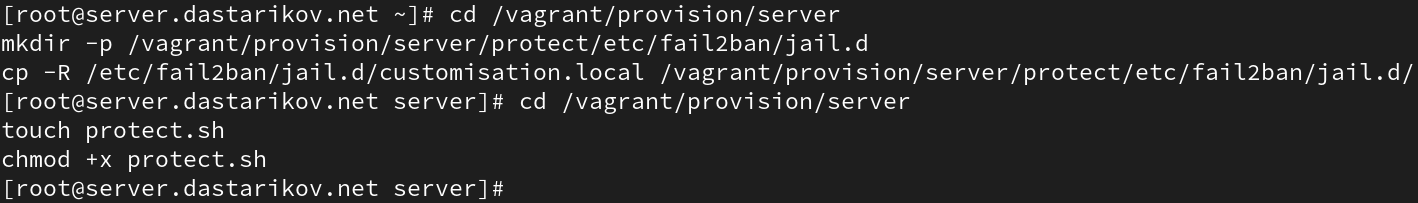
\includegraphics[width=\textwidth]{../images/image18.png}
    \captionof{figure}{Настройка внутреннего окружения сервера.}
\end{frame}

\begin{frame}[fragile]
\frametitle{Внесение изменений в настройки внутреннего окружения виртуальных машин}
\begin{minted}{bash}
    #!/bin/bash
    echo "Provisioning script $0"
    echo " Install needed packages"
    dnf -y install fail2ban
    echo "Copy configuration files"
    cp -R /vagrant/provision/server/protect/etc/* /etc
    restorecon -vR /etc
    echo "Start fail2ban service"
    systemctl enable fail2ban
    systemctl start fail2ban
\end{minted}
\end{frame}

\begin{frame}[fragile]
\frametitle{Внесение изменений в настройки внутреннего окружения виртуальных машин}
\begin{minted}{bash}
    server.vm.provision "server protect",
        type: "shell",
        preserve_order: true,
        path: "provision/server/protect.sh"
\end{minted}
\end{frame}

\begin{frame}
\frametitle{Выводы}
\begin{itemize}
    \item Во время выполнения лабораторной работы получили навыки настройки обеспечения базовой защиты от атак типа "brute force" с помощью программы Fail2ban.
\end{itemize}
\end{frame}
\end{document}
